\section{Two Ray Plane Earth}
In contrast to the Friss pathloss model, the approximated two-ray-ground-reflection path loss model (ATRPL) \citep{two_ray}, considers both the direct wave and the reflected ground wave. Also the ATRPL does not depend on the frequency, as the Friss path loss model does. The received power depending on the distance is given in \eqref{two_ray_model}.

\begin{equation}
P_r(d) = \frac{P_t G_t G_r}{L} \left(\frac{h_t h_r}{d^2}\right)^2
\label{two_ray_model}
\end{equation}

Where $h_t$ and $h_r$ are the heights of the transmitter and receiver antennas respectively. And L is the system loss. A illustration of a scenario of when to use the ATRPL, can be seen on the following Figure.

\begin{figure}[H]
\centering
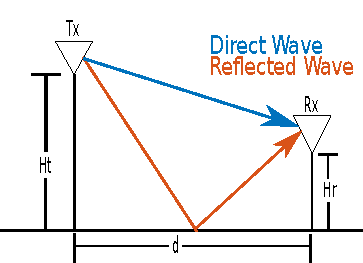
\includegraphics[width=0.5\textwidth]{Figures/two_ray_illu.pdf}
\caption{Illustration of a scenario of when to use the ATRPL model}
\label{two_ray_scena}
\end{figure}


The ATRPL is used if the distance $d$ is greater then a critical point $d_{c}$ given in \eqref{two_ray_cond} if the condition is false then Friss path loss model can be used. 

\begin{equation}
d>d_{c}
\label{two_ray_cond}
\end{equation}

with $d_{c}$ given as:

\begin{equation}
d_{c} = \frac{4\pi \cdot h_t h_r}{\lambda}
\label{critical_fac_dc}
\end{equation}

If the condition is false then interference occur which looks like ripples this is caused by the constructive and destructive combination of the two rays. The ATRPL does not account for this.  

\subsection{Critical point calculation}
For the measurements done, the condition given in \eqref{two_ray_cond} is tested:


\subsubsection{Calculation example for both transmitter and receiver antennas heights at 2 m, at 858MHz}

For 2m and 2m heights of the transmitter antenna and receiver antenna. This for a frequency of 858MHz:

\begin{equation}
d_{c} = \frac{4\pi \cdot 2m \cdot 2m}{0.3494m} = 143.86m
\label{critical_fac_dc_calc_2_2_858MHz}
\end{equation}

So for 2m and 2m, for all distances from 1m to 30m between the sender and the receiver, it is indicated that Friss shall be used. 


Again the condition is not met, for all distances, for 2m and 2m. This means that the ATPL shall not be used.


%\subsubsection{For 2m and 0.34 heights of transmitter and receiver antennas, for both 858MHz and 2.58GHz}
%While when the height of the transmitter antenna is 2m while the receiver antenna is placed at 0.34m, also for a frequency of 858Mhz:

%\begin{equation}
%d_{c} = \frac{4\pi \cdot 2m \cdot 0.34m}{0.3494m} = 24.45m
%\label{critical_fac_dc_calc_2_0.34}
%\end{equation}

%So for 2m and 0.34m for all distances from 1m to 15m, this condition is true while for a distance of 30m this condition is not true.

%While the the same for 2.58GHz:

%\begin{equation}
%d_{c} = \frac{4\pi \cdot 2m \cdot 0.34m}{0.1161m} = 73.60m
%\label{critical_fac_dc_calc_2_0.34.58GHz}
%\end{equation}

%Again this condition is not met for all distances.

%0.01, 0.08, 0.34, 2.

\subsection{Critical point test for 858Mhz}

\textbf{For $h_{r}=0.01m$ set, and $h_{t}= 0.01m, 0.08m, 0.34m, 2m$, $d=1m,2m,4m,8m,15m,30m$}

In the following a \autoref{critical_dc_858_0.01_cond} is made to illustrate if the condition stated in \ref{two_ray_cond_1}, is met for all distances, 1m,2m,4m,8m,15m and 30m, between the transmitter and receiver for the frequency 858MHz with 0.01m set as transmitter height $h_{t}$ while the receiver height positions are $h_{r} = 0.01m, 0.08m, 0.34m, 2m$ .
\\
\\
\begin{table}[H]
\centering
\begin{tabular}{|l|l|l|ll}
\cline{1-3}
                   & 858MHZ &                                                                               &  &  \\ \cline{1-3}
$h_{t}$,$h_{r}$    & Met    & Not met                                                                       &  &  \\ \cline{1-3}
0.01m, 0.01m, $d_{c}$ = 0.0036m        &    & \begin{tabular}[c]{@{}l@{}}At all distances\\ \end{tabular} &  &  \\ \cline{1-3}
0.01m, 0.08m,  $d_{c}$ = 0.028m       &   & \begin{tabular}[c]{@{}l@{}}At all distances\\ \end{tabular}  &  &  \\ \cline{1-3}
0.01m, 0.34m,  $d_{c}$ = 0.12m       &   & \begin{tabular}[c]{@{}l@{}}At all distances\\ \end{tabular}   &  &  \\ \cline{1-3}
0.01m, 2m, $d_{c}$ = 0.72m          &    & \begin{tabular}[c]{@{}l@{}}At all distances\\ \end{tabular}   &  &  \\ \cline{1-3}
\end{tabular}
\caption{Critical distance for 0.01m}
\label{critical_dc_858_0.01_cond}
\end{table}

From the above \autoref{critical_dc_858_0.01_cond} it can be concluded that the ATPL shall be used. This is true as $d>d_{c}$, for all $d$, for all height combinations.


\textbf{For $h_{t} = 0.08m$ set, and $h_{r}= 0.08m, 0.34m, 2m$, $d=1m,2m,4m,8m,15m,30m$}


\begin{table}[H]
\centering
\label{my-label}
\begin{tabular}{|l|l|l|ll}
\cline{1-3}
                   & 858MHZ     &                                                                             &  &  \\ \cline{1-3}
$h_{t}$,$h_{r}$    & Met        & Not met                                                                     &  &  \\ \cline{1-3}
0.08m, 0.08m,$d_{c}$ = 0.23m         &        & \begin{tabular}[c]{@{}l@{}}At all distances\\ \end{tabular} &  &  \\ \cline{1-3}
0.08m, 0.34, $d_{c}$ = 0.97m         &      & \begin{tabular}[c]{@{}l@{}}At all distances\\ \end{tabular} &  &  \\ \cline{1-3}
0.08m, 2m, $d_{c}$ = 5.76m           & 1,2 and 4m  & \begin{tabular}[c]{@{}l@{}}At 8,15 and 30m\\ \end{tabular}  &  &  \\ \cline{1-3}
\end{tabular}
\caption{My caption}
\end{table}

For $h_{t}$=0.08m and $h_{r}$=2m the condition $d<d_{c}$ for distances of 1m, 2m and 4m, is met. This means that the Friss, can be used. While the rest of the time ATPL shall be used.  

%and the results with Two ray model shall not experience oscillations caused by the constructive and destructive combination of the two rays. 


\textbf{For $h_{t}=0.34m$ set, and $h_{r}=0.34m, 2m$, $d=1m,2m,4m,8m,15m,30m$}  

\begin{table}[H]
\centering
\label{my-label}
\begin{tabular}{|l|l|l|ll}
\cline{1-3}
                   & 858MHZ     &                                                                         &  &  \\ \cline{1-3}
$h_{t}$,$h_{r}$ & Met          & Not met                                                                    &  &  \\ \cline{1-3}
0.34m, 0.34m, $d_{c}$ = 4.16m       & 1,2,4       & \begin{tabular}[c]{@{}l@{}}At 8, 15,30m\\ \end{tabular} &  &  \\ \cline{1-3}
0.34m, 2m, $d_{c}$ = 24.48m          & 1,2,4,8,15   & \begin{tabular}[c]{@{}l@{}}At 30\\\end{tabular}       &  &  \\ \cline{1-3}
\end{tabular}
\caption{My caption}
\end{table}

\newpage

\textbf{For $h_{t} = 2m$ set, and $h_{r}=2m$,  $d=1m,2m,4m,8m,15m,30m$}

\begin{table}[H]
\centering
\label{my-label}
\begin{tabular}{|l|l|l|ll}
\cline{1-3}
             & 858MHZ                                                                     &         &  &  \\ \cline{1-3}
$h_{t}$,$h _{r}$ & Met                                                                    & Not met &  &  \\ \cline{1-3}
2m,2m. $d_{c}$ = 144m        & \begin{tabular}[c]{@{}l@{}}At all distances\\  \end{tabular} &         &  &  \\ \cline{1-3}
\end{tabular}
\caption{My caption}
\end{table}

\subsection{Critical point test for 2.58Ghz}

\textbf{For $h_{r}=0.01m$ set, and $h_{t}= 0.01m, 0.08m, 0.34m, 2m$, $d=1m,2m,4m,8m,15m,30m$}

\begin{table}[H]
\centering
\label{my-label}
\begin{tabular}{lllll}
\cline{1-3}
\multicolumn{1}{|l|}{}                                                                         & \multicolumn{1}{l|}{2.58GHz}   & \multicolumn{1}{l|}{}                 &  &  \\ \cline{1-3}
\multicolumn{1}{|l|}{$h_{t}$,$h_{r}$}                                                       & \multicolumn{1}{l|}{Met}       & \multicolumn{1}{l|}{Not met}          &  &  \\ \cline{1-3}
\multicolumn{1}{|l|}{\begin{tabular}[c]{@{}l@{}}0.01m,0.01m\\ $d_{c}$ = 0.010\end{tabular}}   & \multicolumn{1}{l|}{}          & \multicolumn{1}{l|}{At all distances} &  &  \\ \cline{1-3}
\multicolumn{1}{|l|}{\begin{tabular}[c]{@{}l@{}}0.01m, 0.08m\\ $d_{c}$ = 0.0865\end{tabular}} & \multicolumn{1}{l|}{}          & \multicolumn{1}{l|}{At all distances} &  &  \\ \cline{1-3}
\multicolumn{1}{|l|}{\begin{tabular}[c]{@{}l@{}}0.01m,0.34m\\ $d_{c}$ = 0.36\end{tabular}}    & \multicolumn{1}{l|}{}          & \multicolumn{1}{l|}{At all distances} &  &  \\ \cline{1-3}
\multicolumn{1}{|l|}{\begin{tabular}[c]{@{}l@{}}0.01m,2m\\ $d_{c}$ = 2.16\end{tabular}}       & \multicolumn{1}{l|}{1m and 2m} & \multicolumn{1}{l|}{At 4,8,15,30m}    &  &  \\ \cline{1-3}
                                                                                               &                                &                                       &  & 
\end{tabular}
\caption{My caption}
\end{table}


\textbf{For $h_{t} = 0.08m$ set, and $h_{r}= 0.08m, 0.34m, 2m$, $d=1m,2m,4m,8m,15m,30m$}

\begin{table}[H]
\centering
\label{my-label}
\begin{tabular}{lllll}
\cline{1-3}
\multicolumn{1}{|l|}{}                                                                       & \multicolumn{1}{l|}{2.58GHz}                                                   & \multicolumn{1}{l|}{}                                                             &  &  \\ \cline{1-3}
\multicolumn{1}{|l|}{$h_{t}$,$h_{r}$}                                                     & \multicolumn{1}{l|}{Met}                                                       & \multicolumn{1}{l|}{Not met}                                                      &  &  \\ \cline{1-3}
\multicolumn{1}{|l|}{\begin{tabular}[c]{@{}l@{}}0.08m,0.08m\\ $d_{c}$ = 0.69\end{tabular}}  & \multicolumn{1}{l|}{}                                                          & \multicolumn{1}{l|}{At all distances}                                             &  &  \\ \cline{1-3}
\multicolumn{1}{|l|}{\begin{tabular}[c]{@{}l@{}}0.08m, 0.34m\\ $d_{c}$ = 2.94\end{tabular}} & \multicolumn{1}{l|}{1, 2m}                                                     & \multicolumn{1}{l|}{\begin{tabular}[c]{@{}l@{}}At, 4,8,15 and\\ 15m\end{tabular}} &  &  \\ \cline{1-3}
\multicolumn{1}{|l|}{\begin{tabular}[c]{@{}l@{}}0.08m,2m\\ $d_{c}$ = 17.31\end{tabular}}    & \multicolumn{1}{l|}{\begin{tabular}[c]{@{}l@{}}1,2,4,8\\ and 15m\end{tabular}} & \multicolumn{1}{l|}{At 30m}                                                       &  &  \\ \cline{1-3}

\end{tabular}
\caption{My caption}
\end{table}

\textbf{For $h_{t}=0.34m$ set, and $h_{r}=0.34m, 2m$, $d=1m,2m,4m,8m,15m,30m$}  


\begin{table}[H]
\centering

\label{my-label}
\begin{tabular}{lllll}
\cline{1-3}
\multicolumn{1}{|l|}{}                                                                       & \multicolumn{1}{l|}{2.58GHz}                                                    & \multicolumn{1}{l|}{}           &  &  \\ \cline{1-3}
\multicolumn{1}{|l|}{$h_{t}$,$h_{r}$}                                                     & \multicolumn{1}{l|}{Met}                                                        & \multicolumn{1}{l|}{Not met}    &  &  \\ \cline{1-3}
\multicolumn{1}{|l|}{\begin{tabular}[c]{@{}l@{}}0.34m,0.34m\\ $d_{c}$ = 12.51\end{tabular}} & \multicolumn{1}{l|}{\begin{tabular}[c]{@{}l@{}}At 1,2,4\\ and 8m\end{tabular}}  & \multicolumn{1}{l|}{At 15, 30m} &  &  \\ \cline{1-3}
\multicolumn{1}{|l|}{\begin{tabular}[c]{@{}l@{}}0.34m, 2m\\ $d_{c}$ = 73.6\end{tabular}}    & \multicolumn{1}{l|}{\begin{tabular}[c]{@{}l@{}}At all\\ distances\end{tabular}} & \multicolumn{1}{l|}{}           &  &  \\ \cline{1-3}
\end{tabular}
\caption{My caption}
\end{table}


\textbf{For $h_{t} = 2m$ set, and $h_{r}=2m$,  $d=1m,2m,4m,8m,15m,30m$}

\begin{table}[H]
\centering

\label{my-label}
\begin{tabular}{lllll}
\cline{1-3}
\multicolumn{1}{|l|}{}                                                                 & \multicolumn{1}{l|}{2.58GHz}                                                     & \multicolumn{1}{l|}{}        &  &  \\ \cline{1-3}
\multicolumn{1}{|l|}{$h_{t}$,$h_{r}$}                                               & \multicolumn{1}{l|}{Met}                                                         & \multicolumn{1}{l|}{Not met} &  &  \\ \cline{1-3}
\multicolumn{1}{|l|}{\begin{tabular}[c]{@{}l@{}}2m,2m\\ $d_{c}$ = 432.9\end{tabular}} & \multicolumn{1}{l|}{\begin{tabular}[c]{@{}l@{}}At all \\ distances\end{tabular}} & \multicolumn{1}{l|}{}        &  &  \\ \cline{1-3}
\end{tabular}
\caption{My caption}
\end{table}

%else will the received power theoretically oscillates between
%local maxima of 6dB above free space to $-\infty$ dB at local minima.

%\subsubsection{Power vs distance} 

%\subsubsection{Propagation path}

%The path can be divided into three segments the first being if:

%\begin{equation}
%d<h_{t}
%\end{equation}

%If this condition is true then:

%\begin{itemize}
%The two rays add constructively
%Path loss is slowly increasing 
%\end{itemize}




%LPE = 40 log10(d) $-$ 20 log10(ht) $-$ 20 log10(hr )







%\begin{table}[H]
%\centering
%\label{mylabel}
%\begin{tabular}{|l|l|l|ll}
%\cline{1-3}
 %               & 858MHz        &                                                                                   &  &  \\              \cline{1-3}
%$h_{t}$,$h_{r}$ & Not met & Met                                                                           &  &  \\ \cline{1-3}
%0.01m, 0.01m       & At all distances               & \begin{tabular}[c]{@{}l@{}}\\ $d_{c}$ = 0.0036m\end{tabular}   &  &  \\ \cline{1-3}
%2m, 0.34m          & 30m           & \begin{tabular}[c]{@{}l@{}}All other distances\\ $d_{c}$ = 24.45m\end{tabular} &  &  \\ \cline{1-3}
%2m, 0.08m          & 8m, 15m, 30m  & \begin{tabular}[c]{@{}l@{}}At 1m, 2m, 4m\\ $d_{c}$ = 5.76m\end{tabular}        &  &  \\ \cline{1-3}
%2m, 0.01m          & All distances & $d_{c}$ = 0.72m                                                                &  &  \\ \cline{1-3}
%\end{tabular}
%\caption{Table illustrating if the condition given in \ref{two_ray_cond_1}, is met. This is where 2m is set, with 0.34m,0.08m and 0.01m where it is set for which distances the condition is true.}
%\end{table}
